\section{My Contribution}

\subsection{Fitting algorithm for SMPreSS}

The SMPreSS technique works by fitting timecourses of counts of single molecules.  The equation to which it is fit gives estimates of the model parameters.  Francois Robin and myself worked to devise the form of the model equation to be fit. Francois created one simplification for computation, and I found another one that was easier to use.  I implemented the fitting function and implemented techniques to extract the error estimates from the curve fitting results in MATLAB.  This code was delivered with the resulting paper.

\subsection{Control experiments to determine the accuracy of SMPreSS}

Using the SMPreSS technique, we believed it was possible to independently measure the disassociation constant and the photobleaching rate of the system.  To test this, Francois and I set out to systematically vary the laser intensity and determine if our fitting scheme found changes in the photobleaching rate, but not the disassociation constant.  I collected and processed the majority of the data for these control experiments, which found, indeed, that the photobleaching rate varied linearly with laser intensity while the disassociation constant remained constant.

\subsection{Taking the proper mean for Par-3 measurments}

We wished to use measurements of Par-3 disassociation constants as a benchmark with which to compare our technique to the literature.  Originally, the group was taking a pure mean of single molecule lifetime over the total number of events, which led to an estimate of the lifetime that was far shorter than what had been measured previously by FRAP.  The problem was simply that the way we were taking the mean was technically incorrect.  In a given period of time, many more particles with a short lifetime will appear compared to relatively few with a long lifetime.  Meanwhile if you were to observe at a single instance, there would be closer to an exponential distribution of short and long time events. Taking the average over a wide swath of time therefore, skews the measurement to including more and more short duration events while only counting the long duration events once (even though they appear in many time bins).

The correct way to take the mean is to weight the appearance duration of each event by the duration of the event.  Another way to put this is that you only want to add the mean of the long time over and over for every observed timepoint that you have.  After I incorporated this correction, our measurement lined up with previous measurements for the disassociation constant for Par-3, and we were able to publish this result as a corroboration of our technique's validity.

\section{Introduction}
 
 Dynamic remodeling of the embryonic cell surface is essential for the control of cell polarity, division, shape change and movement during early development. This remodeling involves the dynamic interplay of local exchange and movement of proteins that reside at the interface between the plasma membrane and the actin-rich cell cortex. However, quantifying these processes in embryonic cells remains a significant challenge. One promising approach is single molecule imaging combined with single particle tracking (SPT), which can yield quantitative measurements of local mobilities, binding states and exchange kinetics that are inaccessible to ensemble measurements (1-3). Combining these approaches with powerful genetic tools in a classical model organism could be a powerful way to investigate subcellular dynamics in embryonic cells, but this has yet to be achieved.
 
 
 One key limitation has been the lack of simple and reliable methods for tunable and non-invasive labeling of target molecules. Optimal labeling densities are different for each target and must balance the need for high-density sampling of molecular behavior in space and time against practical requirements for accurate and unbiased single molecule detection and tracking. Methods based on microinjection of fluorescently labeled probes (4,5), or transfection using crippled promoters (6-9) are cumbersome and inherently hard to optimize. Methods based on surface labeling of transmembrane proteins (10-13) may be easier to tune, but cannot be generalized to intracellular targets. A more promising approach for intracellular targets uses genetically encoded photoswitchable fluorescent protein fusions to create a renewable supply of single molecules (14-16), However, this approach does not report on spatiotemporal variations in density or assembly/binding kinetics of the endogenous protein. Moreover, its use in C. elegans would require de novo creation of a transgenic strain for each new target of interest.
 
 
 Here we describe a simple, versatile and minimally invasive method for single molecule imaging at the cell surface in C. elegans embryos that can be applied to any of the large and growing collection of transgenic strains expressing GFP-tagged fusion proteins (17). We combine sequence-specific inhibition of GFP transgene expression with selective photobleaching and simple in vivo standards to achieve and verify single molecule densities of GFP-fusions over normal levels of the endogenous protein. We exploit the intrinsic exchange dynamics of surface-associated proteins to obtain long term (> 5000 frames) sampling of single molecule trajectories at signal-to-noise ratios (SNR), frame rates and densities that can be optimized to measure local mobility and turnover for a given molecule. In particular, we show how these data can be used to extract quantitative information about surface density and turnover through two complementary methods: The first involves direct inference from single particle trajectories. The second method, which we refer to as smPReSS for single molecule Photobleaching Relaxation to Steady State, estimates turnover rates by fitting simple kinetic models to measurements of single molecule densities over time and is therefore insensitive to particle tracking errors. To demonstrate the power of this approach, we quantify spatiotemporal variations in mobility and turnover for the polarity protein Par-6 and for actin filaments during asymmetric cell division in the one-cell C. elegans embryo.
 
 \section{Results}
 
 \subsection{Obtaining and verifying single molecule levels for any GFP fusion protein.}
 
 In C. elegans, a 200nm thick eggshell (18,19) makes it difficult to image subsurface dynamics with true TIRF optics. To overcome this, we used near-TIRF illumination (20), optimizing laser angle and intensity to achieve ~even illumination across the field of view while maintaining adequate SNR for robust single particle detection and tracking (Fig. \ref{fig:fig1}a; Supplementary Fig. \ref{fig:fig1}; below and Supplementary Note 6). For any given transgenic strain expressing GFP fused to a target protein, we used a two-step method to achieve densities of GFP-tagged proteins suitable for single molecule imaging (Fig. \ref{fig:fig1}b). First, we directed RNA interference (RNAi) against the GFP sequence to selectively reduce maternal expression of the transgene, yielding low levels of GFP-tagged protein over normal levels of the endogenous protein. For more than a dozen strains tested, we could readily tune exposure times to obtain transgene expression levels at which diffraction limited-speckles could be observed at the cell surface by near-TIRF microscopy (Fig. \ref{fig:fig1}c, bottom). In a second step, we used photobleaching to further reduce speckle densities (\#speckles/µm2) and mean speckle intensity towards single molecule levels (Fig. \ref{fig:fig1}d), with no adverse consequences for cell viability (see Supplementary Note 4).
 
 
 

 \begin{figure}[h!]
 	\centering
 	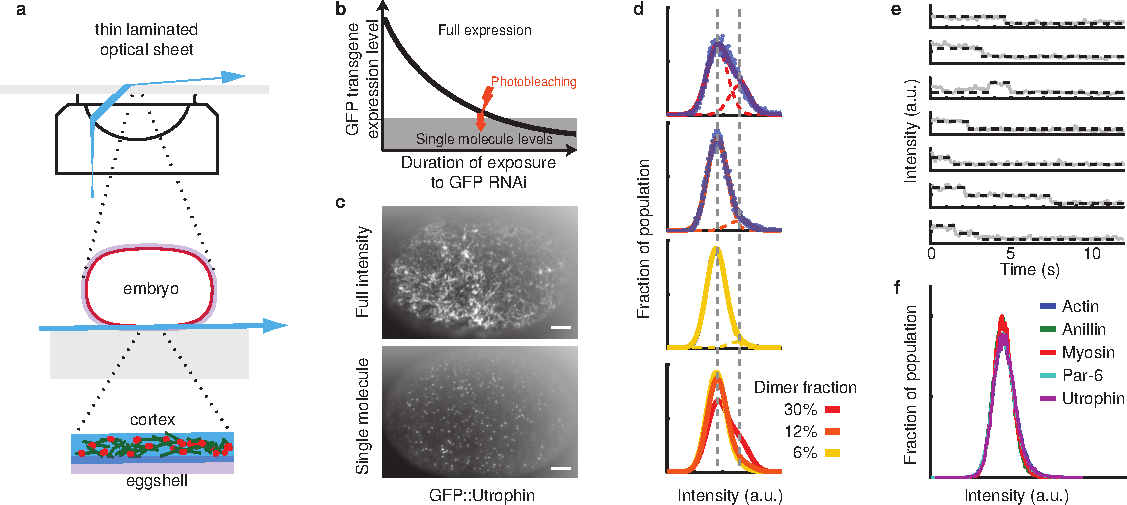
\includegraphics[width=\hsize]{nmeth/Fig1}
 	\caption{\label{fig:fig1} Imaging single molecules at the cortex in living embryos. (a-c) Schematic overview of the Near-TIRF imaging approach. (a) Top: Incident laser angle at the cover glass/specimen interface is tuned to create a thin and narrowly inclined laminar sheet (blue) of laser light. At cell (middle) and subcellular (bottom) scales, the laminar sheet is nearly parallel to the coverslip/specimen interface, and is thick enough to illuminate the entire cell cortex in the field of view. (b) Basic approach to achieve single molecule levels for any GFP-fusion strain in C. elegans, using a combination of RNAi against GFP and photobleaching. (c) Near-TIRF micrographs of a one-cell embryo expressing GFP::Utrophin showing full intensity and single molecule levels. Scale bar = 5 µm. (d) Distribution of intrinsic speckle intensities (average particle intensity - local average background) in a strain expressing GFP::PAR-1 for a range of depletion levels. Fits to a sum of two Gaussians representing one and two-molecule speckles measure a decrease in the proportion of doublets from 12\% to 5\%. Bottom panel compares directly all three previous panels. Images were obtained using identical imaging conditions. (e) Direct verification of single molecule levels by single step photobleaching in an embryo expressing GFP::Actin. Multiple step photobleaching can be readily detected at higher expression levels (last two panels). (f) Intrinsic speckle intensity at low particle densities is essentially identical across all GFP strains tested.}
 \end{figure}
 
 
 
 Next we established a general method to verify single molecule levels for any GFP fusion strain that can be readily extended across labs and imaging platforms. We focused on polarity maintenance phase in the one-cell embryo when the densities and distributions of many surface proteins are essentially stationary. Concentrating initially on a strain expressing GFP::Actin, we reduced transgene levels as above until the average intrinsic speckle intensity (Iint = Ispeckle - Ibackground) reached a minimum value and the distribution of intensities was well-fit by a single Gaussian (Fig. \ref{fig:fig1}d). Then we imaged at high laser power such that speckle disappearance was dominated by photobleaching, rather than disassembly. Under these conditions, the majority of disappearance events occurred in single-steps, confirming that the minimum intensity speckles we observe correspond to single GFP molecules (Fig. \ref{fig:fig1}e). Strikingly, when we reduced expression levels in 5 other GFP fusion strains to minimize the mean speckle intensity, we measured speckle intensity distributions during maintenance phase that were indistinguishable from one another and from those measured for GFP::Actin under the same imaging conditions (Fig. \ref{fig:fig1}f). Moreover, by fitting multiple Gaussians (for 1,2,…N fluorophores/particle) to the distribution of Iint, we could readily detect when more than 5\% of speckles contain multiple fluorophores (Fig. \ref{fig:fig1}d, Supplementary Fig. \ref{fig:fig3}a). Thus for any given strain, it is possible to pinpoint a characteristic speckle density below which a “pure” population of single molecules can be reliably observed, which can subsequently be used to calibrate single molecule imaging on other platforms.
 
 
 \subsection{Exploiting intrinsic exchange kinetics to achieve optimized sampling of single molecule mobility and turnover}
 
 We sought to exploit the intrinsic exchange dynamics of surface-associated proteins to create a self-renewing pool of GFP-tagged single molecules at the cell surface that could be followed over time to measure mobility and turnover. To establish a kinetic basis for this approach, we consider a GFP-tagged protein that exchanges dynamically between the bulk cytoplasm and a region of the cell surface, which is observed by near-TIRF microscopy (Fig. \ref{fig:fig2}a). The number of molecules N(t) within this region over time is governed by:
 
 
 (1)
 
 where kapp is an observable appearance rate that depends on the cytoplasmic concentration of GFP-tagged protein (kapp = kon × Y, where Y is the cytoplasmic concentration) and the nature of the binding process, and koff and kph are pseudo-first order rate constants such that koff x N is the rate (in molecules per second) at which particles disappear due to unbinding or disassembly, and kph x N is the rate (in molecules per second) at which they disappear due to irreversible photobleaching. (Fig. \ref{fig:fig2}a). Prior to illumination, kph = 0 and the steady state density is . During illumination, kph becomes non-zero; if the cytoplasmic pool were infinite, the system would approach a new steady state density given by , which is a fixed fraction of the initial unobserved value (Fig. \ref{fig:fig2}b). In practice, irreversible photobleaching will gradually deplete a finite cytoplasmic pool. A variant of the kinetic model that accounts for this depletion (see Supplementary Note 8) predicts a biphasic response to the onset of illumination: a fast relaxation towards ~ , followed by a slower decay towards 0, at a rate which depends on the photobleaching rate and the size of the cytoplasmic pool (Fig. \ref{fig:fig2}b). For a given target molecule, koff is fixed. However, kph depends on imaging conditions (i.e. the intensity and duty ratio of the laser illumination, while kapp can be adjusted by tuning the initial size of the GFP-tagged pool. Thus by co-tuning these factors, it should be possible to target a desired density at quasi-steady state for a range of imaging conditions.
 
 
 
 \begin{figure}[h!]
 	\centering
 	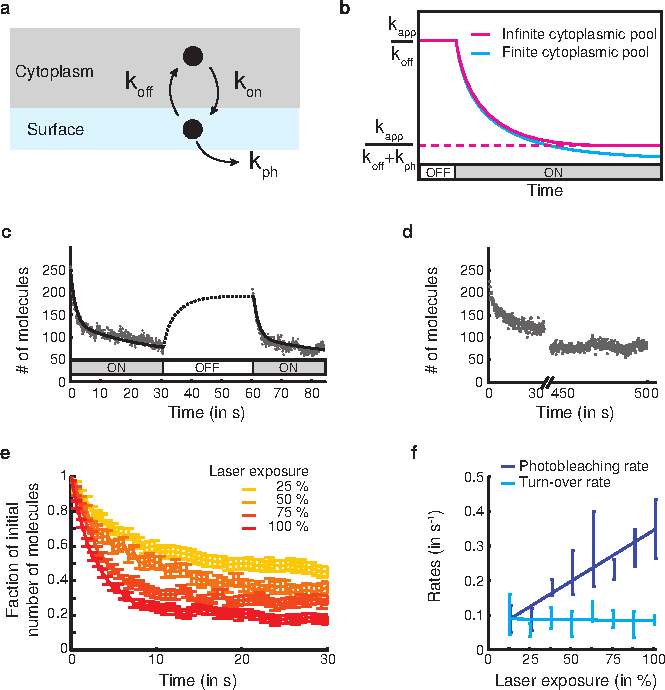
\includegraphics[width=0.6\hsize]{nmeth/Fig2}
 	\caption{\label{fig:fig2} Exploiting dynamic exchange between cytoplasm and cell surface to obtain long-term tunable and high-density sampling of single molecule behaviors. (a) The basic kinetic principle: During imaging, the level of surface-associated proteins is set by a dynamic balance of: appearance (binding or assembly) at an observable rate kapp, disappearance (unbinding or disassembly) at a per-molecule rate koff, and photobleaching at a per molecule rate kph. (b) The predicted response o f an initially unobserved cell at steady state to a step change in illumination. For an infinite cytoplasmic pool (), the surface density relaxes to a new illuminated steady state. For a finite cytoplasmic pool (), fast relaxation is accompanied by a slower decay caused by irreversible photobleaching. (c) Biphasic response for GFP::Actin under illumination conditions that allow accurate single molecule detection and tracking. () real data; () model fit; () discontinuous jump from t = 30s to t = 450s. (d) The fast relaxation to a quasi-stable density during illumination is rapidly reversed when the laser is turned off. (e) Surface density vs time at various laser exposures, shown as a fraction of the initial unobserved density. Error bars indicate standard error of the mean (n=7,9,6,7). (f) Estimates of per molecule disappearance (koff) and photobleaching (kph) rates as a function of laser exposure. Error bars indicate standard deviation, (n=12,7,8,9,7,6,7,7). Solid lines show a linear regression against the data. kph increases linearly with laser exposure, while koff remains constant. 100\% laser power ~ 1.6µW/µm2.}
 \end{figure}
 
 
 
 
 
 To test this approach, we chose two representative strains expressing GFP::Actin and PAR-6::GFP. Actin monomers exchange dynamically with the cell surface through local filament assembly and disassembly, and based on previous work, we expected GFP::F-Actin to be relatively immobile at the cell surface and to turn over in a few 10s of seconds (see 21 for review), while fast-diffusing monomers of GFP::Actin should produce highly blurred images and thus escape detection under our imaging conditions (6). Par-6 is a conserved polarity protein that binds dynamically to sites on the plasma membrane (22-24) and recent FRAP measurements suggest that it diffuses rapidly at the cell surface and dissociates very slowly, with an effective dissociation rate constant koff = 5.4 ± 5 × 10-3 s -1 (25). Focusing again on polarity maintenance phase, we reduced densities to single molecule levels, allowed the system to equilibrate unobserved, and then recorded data for a range of laser intensities and exposure times (Fig. \ref{fig:fig2}c-e, Supplementary Fig. \ref{fig:fig3}b). For both strains, we observed the predicted biphasic response to a step change in illumination - a rapid initial decrease in the number of molecules to a quasi-stable value followed by slower decay (Fig. \ref{fig:fig2}c,d, Supplementary Fig. \ref{fig:fig2},3a, also Supplementary Video 1). Importantly, the initial decrease was reversed with equally rapid kinetics when the laser was turned off (Fig. \ref{fig:fig2}c) confirming that the quasi-steady state is set by a dynamic balance of exchange and photobleaching. For both strains, we could therefore obtain robust estimates for effective dissociation and photobleaching rate constants koff and kph, by fitting the predicted biphasic kinetics to the change in single molecule density over time; for each strain, we optimized fitting conditions by adjusting laser exposure (intensity and duty ratio; see below and Supplementary Note 9). As expected, estimates of kph varied linearly with laser exposure while estimates of koff remained fixed over a range of exposures (Fig. \ref{fig:fig2}f). Significantly, our estimates of koff for Par-6 in the anterior cortex (koff =7.4 ± 0.7 ×10-3 s-1) are consistent with those previously obtained by FRAP (koff = 5.4 ± 5 ×10-3 s-1, 25). We refer to this approach as smPReSS for single-molecule Photobleaching Relaxation to Steady State. Because smPReSS relies directly on counting single molecules, it is relatively insensitive to non-specific fluorescence and can be applied at very low fluorophore densities that would be inaccessible using ensemble methods like FRAP and its variants. Moreover, because it does not rely on particle tracking, it is insensitive to particle tracking errors.
 
 
 Next, we assessed the potential for long-term high-density sampling of single molecule trajectories, as previously achieved with photoswitchable fluorophores. To this end, we set laser intensities to ensure signal-to-noise ratios and frame rates suitable for robust particle tracking using standard SPT algorithms and software (Supplementary Video 1-3, 26, 27, Supplementary Note 6, Supplementary Table 1). Under these conditions, we measured effective photobleaching rate constants kph ~ 0.1 s-1 for GFP::Actin and kph ~ 0.3 s-1 for PAR-6::GFP, resulting in less than 30\% loss in density over 5000 frames (Fig. \ref{fig:fig2}d, Supplementary Fig. \ref{fig:fig2}, 3a). When we pre-tuned the initial size of the cytoplasmic pool to optimize quasi-stable densities towards maximal values consistent with robust SPT, we were able to recover for GFP::Actin (resp. PAR-6::GFP) ~30,000 (resp. ~7,500) individual trajectories over the 5000-frame interval, with an average duration of 35 (resp. 15) frames, and ~5000 (resp. ~250) trajectories lasting longer than 80 frames. We observed comparable results with several other strains (data not shown). Thus, the intrinsic exchange dynamics of GFP-tagged proteins can be exploited to achieve continuous long-term single molecule imaging, and these imaging conditions can be tuned to optimize single particle tracking analysis or estimates of bulk turnover by smPReSS.
 
 
 \subsection{SPT analysis reveals distinct classes of Par-6 mobility during maintenance phase}
 
 The ability to rapidly sample large numbers of individual trajectories makes it possible to analyze surface dynamics during well-defined and short-lived windows of developmental time. To illustrate this, we tracked local movements of PAR-6::GFP molecules at the cell surface during maintenance phase in one-cell embryos. To get a rough classification of Par-6 mobilities, we measured mean-square-displacement (MSD) vs lag time τ for 1086 trajectories with lifetimes larger than 80 frames (Fig. \ref{fig:fig3}a,b). Then we fit the first 10 time points to MSD = 4Dτα to estimate the anomalous diffusion exponent α and a short-term diffusivity D. This analysis revealed what appears to be at least two distinct mobility classes (Fig. \ref{fig:fig3}b,c, Supplementary Video 1,4,5). Approximately 43\% of Par-6 molecules undergo what appears to be simple diffusion, with 0.9<α<1.2 and short term diffusivity D = 0.17 ± 0.10 µm2.s-1 (red traces and dots in Fig. \ref{fig:fig3}b,c), which is comparable to previous measurements by FRAP (0.28 ± 0.05 µm2.s-1, 25). Another ~22\% of Par-6 molecules undergo what appears to be slower sub-diffusive motion, with α<0.6 and short term D = 0.008 ± 0.008 (blue traces and dots in Fig. \ref{fig:fig3}b,c). The remaining 35\% of the tracks undergo intermediate behavior, with short term D = 0.057 ± 0.032 for 0.6 ≤ α ≤ 0.9 (gray traces and dots in Fig. \ref{fig:fig3}b,c). Simulating Brownian diffusion for 177 particles with diffusivities chosen randomly from the range D = 0.15 ± 0.05 µm2.s-1 and then analyzing trajectories as above reproduced a distribution of short term D and alpha values very similar to the distribution observed for the subset of real particles with 0.9<α<1.2 (Fig. \ref{fig:fig3}d). In contrast (and as expected) for no values of D did simulated Brownian diffusion reproduce the class of trajectories for α<0.6 observed for single molecules of Par-6 (Supplementary Fig. \ref{fig:fig4}). These observations are consistent with previous studies documenting two populations of Par-6, punctate and diffuse, with distinct localizations and genetic requirements, and which likely reflect different binding modes and binding partners for Par-6 (22). Further analyses combining the sampling methods introduced here with e.g. Bayesian trajectory analysis (28,29) and genetic manipulation should yield further information about these different binding states and their regulation.
 
  \begin{figure}[h!]
  	\centering
  	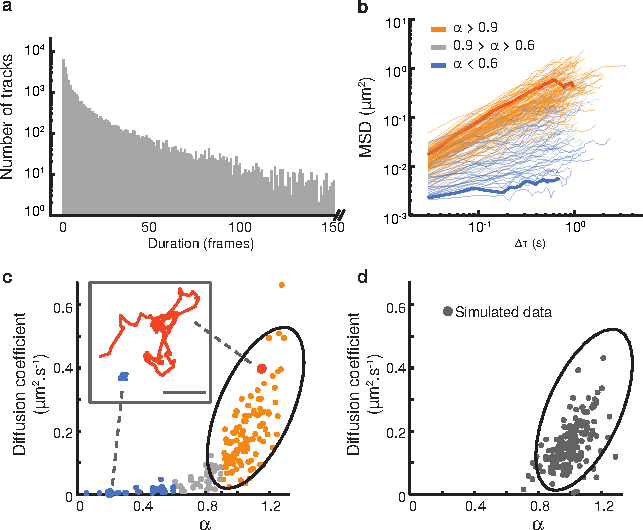
\includegraphics[width=0.8\hsize]{nmeth/Fig3}
  	\caption{\label{fig:fig3}Analysis of PAR-6::GFP mobility during maintenance phase (a) Distribution of track lengths for 30,558 tracks from n = 5 movies taken in one-cell embryos during maintenance phase. (b) Log/log plot of MSD versus lag time (∆τ) for all 177 tracks with length ≥ 80 frames extracted from one of the movies, reveals what appears to be a mixture of brownian and anomalous diffusion. Traces have been assigned colors based on slope (α),(): α<0.6; (): 0.6<α<0.9; (): α>0.9 (c) Scatter plot of diffusion coefficient D versus exponent α, measured by fitting MSD = 4Dtα for the first 10 lag times of the tracks shown in (b), with (): α<0.6; (): 0.6<α<0.9; (): α>0.9 . Inset shows two particular trajectories drawn from opposite ends of the scatter plot and indicated by colored circles. Scale bar, 1µm. (d) Scatter plot for 177 trajectories obtained by simulating pure brownian diffusion for ≥ 80 frames with D = 0.15+/- 0.05 µm2.s-1 and measuring D and α as in (c). () simulated tracks. Note the close match to experimental data for 0.9 < α < 1.2, but the failure to match points at the bottom left (low D and α). }
  \end{figure}
 

 
 
 \subsection{Measuring spatial and temporal variations in density and turnover}
 
 A key advantage of our approach is that the GFP-tagged proteins sample the same kinetics as the underlying pool. Thus, they report not just on mobilities, but also on spatiotemporal variation in densities, appearance rates (kapp) and per molecule turnover rates (koff). In principle, kapp and koff can be measured either directly from single molecule trajectories or by smPReSS as described above. However practical considerations constrained the choice of method as illustrated by analysis of Par-6 turnover during polarity maintenance and actin turnover during cell division.
 
 
 \subsection{Measuring spatial variation in Par-6 turnover during maintenance phase.}
 
 Par-6 is highly enriched at the anterior cortex in polarized one-cell embryos. These differences are thought to be caused by more rapid dissociation of Par-6 in the posterior (30). However, anterior vs posterior differences in dissociation rate cannot be detected by conventional FRAP analysis because the densities of Par-6 in the posterior are too low. Unfortunately, the photobleaching rates (kph ~ 0.3 s-1) required for accurate particle tracking are ~40-fold higher than the dissociation rates (koff =7.4 ± 0.7 × 10-3 s-1) measured by smPReSS. Thus resolving A vs P differences in turnover by particle tracking would be difficult or impossible because photobleaching will dominate small differences in koff. Instead, we exploited the tunability of our approach, setting laser exposure and image acquisition (100\% laser, 30ms exposure at 1 second intervals) to maintain accurate detection while reducing photobleaching rates to kph ~ 0.005. Under these conditions, smPReSS yielded robust estimates of koff for anterior and posterior regions (, ). Combined with measurements of relative density (), this allowed us to infer relative values for kapp (). Interestingly, our results suggest that the majority of the A vs P difference in density is due to differences in recruitment rates, consistent with the enrichment of several known binding partners for Par-6 (Cdc-42 and Par-3) at the anterior (31,22).
 
 
 
 \begin{figure}[h!]
 	\centering
 	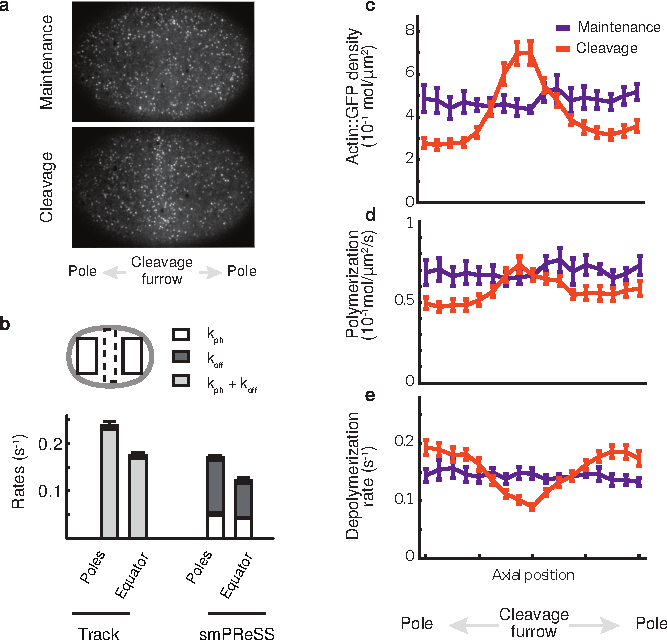
\includegraphics[width=0.8\hsize]{nmeth/Fig4}
 	\caption{\label{fig:fig4} Spatial and temporal analysis of actin dynamics in nmy-2 RNAi embryos. (a) Near-TIRF micrographs of GFP::Actin during maintenance phase (top) and cleavage (bottom). (b) Measurements of turnover at the equator and poles during anaphase using tracking (left) or smPReSS (right). Schematic at top left indicates the equatorial () and polar () regions in which the measurements were made. For tracking, the sum of koff and kph is displayed (); for smPReSS, the values for kph () and koff () are stacked. (c-e) Spatial variation in actin density and turnover kinetics during maintenance phase () and cleavage (), measured by tracking and binned along the antero-posterior axis. (c) cortical density, (d) polymerization rate; (e) depolymerization rate (instantaneous disappearance rate minus estimated photobleaching rate). In b-e, error bars indicate cell to cell SEM (n=7,16). }
 \end{figure}
 
 
 
 \subsection{Spatiotemporal modulation of actin assembly and turnover during cell division}
 
 As a second example, we measured spatiotemporal modulation of actin assembly and disassembly during the first cell division (Fig. \ref{fig:fig4}a, Supplementary Video 2,3). Both actin assembly and disassembly are thought to be modulated during cytokinesis (32), but their relative contributions to actin filament accumulation are not well understood. We performed these experiments in embryos depleted of non-muscle Myosin II to remove the confounding effects of surface deformations and flow and remove myosin-dependent effects on turnover (33,34). We verified strong depletion of Myosin II by the complete failure of cytokinesis and a complete absence of local surface deformation and cortical flow during early anaphase. In the case of GFP::Actin, the turnover rates measured by smPReSS (koff ~ 0.1 s-1) were similar to the photobleaching rates (kph ~ 0.1 s-1) required for accurate particle tracking, and agreed well with estimates of koff from particle tracking (Fig. \ref{fig:fig4}b; Supplementary Fig. 5), suggesting that in this case, we could use SPT to measure spatiotemporal variations in turnover, using the smPReSS measurements of kph to correct for photobleaching. We measured roughly uniform values for kapp and koff along the AP axis during maintenance phase (Fig. \ref{fig:fig4}c-e), consistent with a lack of cortical asymmetry at this stage in myosin-depleted embryos (data not shown). During the transition into anaphase, when the contractile ring normally assembles, we observed a net increase in actin density at the equator as anticipated, and we also observed a net decrease at the poles (Fig. \ref{fig:fig4}a,c). Surprisingly, these changes involved strong modulation of both filament assembly and disassembly (Fig. \ref{fig:fig4}d,e). The equatorial increase was associated with a small increase in assembly rate and a larger decrease in turnover, while the polar decrease in density was associated with both a decrease in assembly and an increase in turnover. Thus our ability to simultaneously resolve assembly, disassembly and density revealed an unappreciated dimension to the control of cortical microfilaments during cell division.
 
 
 \section{Discussion}
 
 Here we describe for the first time a simple and tunable method to monitor single molecule mobility and exchange dynamics at the cell surface in embryonic cells of a genetic model organism - C. elegans. By tuning the size of the GFP-tagged pool and photobleaching rates, we obtained continuous long term sampling of single molecule trajectories at densities and track lengths that are limited mainly by the photostability of GFP and by well-known constraints on the accurate detection and tracking of single molecules. We focused here on single molecule imaging and analysis. However brighter (multi-molecule) speckles may be optimal for some analyses (35), and can be readily achieved through a slightly different tuning of the cytoplasmic pool. Our approach is minimally invasive because it relies on sampling very low levels of GFP fusions over normal levels of the endogenous protein, with no detectable phototoxicity, even at very high laser power. Because we rely on the intrinsic exchange of GFP fusion proteins between the cytoplasm and the cell surface, no additional methods or reagents are required to target fluorophores to the protein of interest, and the method can be readily implemented by anyone with access to a TIRF microscope equipped for GFP excitation and a sufficiently sensitive (e.g. back-thinned EM-gain CCD) camera.. Our approach thus leverages the large collection of existing fusion strains in C. elegans (17), plus recently developed methods for the rapid production of new strains by genome editing (36), and can be readily combined with any of the large arsenal of molecular genetic tools available in this model organism.
 
 
 Our approach is immediately compatible with a growing array of tools, based on SPT, to analyze local heterogeneity and spatiotemporal variation in mobility and binding states (28,29). Under conditions in which photobleaching rates do not dominate turnover (e.g. low mobility and fast turnover as for GFP::Actin), it is possible to measure spatiotemporal variation in turnover directly from single particle trajectories. As an alternative, we introduced a new method called smPReSS that estimates bulk turnover rates by fitting single molecule counts vs time to kinetic exchange models. smPReSS relies only on single molecule detection and thus is insensitive to particle tracking errors. As illustrated by our analysis of Par-6 turnover, smPReSS can be tuned to measure turnover rates under conditions that are inaccessible to SPT analysis or to ensemble-based measurements like FRAP and its variants. A key assumption underlying both approaches is that the kinetics remain stationary during the time it takes to measure them; the validity of this assumption must be assessed on a case-by-case basis.
 
 
 Finally, we developed and optimized the methods described here for use in C. elegans. However sequence specific inhibition of GFP expression in transgenic strains expressing GFP fusions proteins could be implemented in other model organisms through a variety of methods, in particular RNA interference and targeted protein degradation. Likewise, the use of intrinsic turnover to sample single molecule dynamics is a general principle that could be readily applied in other organisms and cell types. Combining these methods with molecular genetic tools already available in model organisms offers a promising new avenue to study cell surface dynamics in developing embryos.